
The local memory interconnect is responsible for routing requests from the
CPU to the appropriate peripheral.
It also enforces the first stage of the SoC memory map
(Table \ref{tab:memory-map:1}).
Figure \ref{fig:design:soc-local-ic} shows a block diagram of how
requests from the CPU are routed to inner layer peripherals.

\begin{itemize}[noitemsep]
\item Local RAM/ROM accesses have 1 cycle access latency.
\item AXI4-Lite bridge requests have a minimum 2 cycle latency for 
      reads and writes.
\end{itemize}

The AXI port is optimised for low resource usage and simplicity.
All requests block until they are completed. There is no
tracking of outstanding requests.

The local interconnect is responsible for returning error responses
when a request is made to unmapped addresses.
This is done using a {\em stub} peripheral, which unmapped address
requests are always routed too.
The stub peripheral then always returns an error response.
There is a single stub peripheral for each CPU requestor interface.

Note that as per the multi-level memory map (\SECREF{design:memory-map}),
it is possible for a 1st level request to map correctly to the AXI4-Lite
bus bridge, but then map to a hole in the memory space.
In this case, the outer layer memory interconnect is responsible for
returning with an error, which is then passed back to the CPU by
the AXI4-Lite bus bridge.

All RTL code for the local memory interconnect is found in
\SOCDIR{rtl/ic}.
A brief description of each module is:
\begin{itemize}

\item \SOCMODULE{ic\_top} - 
    The top level module for the local memory 
    i terconnect. Glues together all of the other modules.

\item \SOCMODULE{ic\_addr\_decode} -
    Responsible for mapping addresses onto the correct peripheral,
    or indicating an unmapped part of the address space has been requested.

\item \SOCMODULE{ic\_cpu\_bus\_bram\_bridge} -
    Converts between the CPU request/response channel based bus and a
    BRAM memory interface.
    Used to communicate with the RAM and ROM local memories.

\item \SOCMODULE{ic\_cpu\_bus\_axi\_bridge} -
    Converts between the two CPU request/response channels and the 5 channel
    AXI4-Lite bus protocol.
    See \SECREF{design:axi-bridge} for more information.

\item \SOCMODULE{ic\_err\_rsp\_stub} - 
    A dummy peripheral which always returns an error response.
    Any requests which do not map to a valid part of the address space are
    mapped to this peripheral.

\item \SOCMODULE{ic\_rsp\_router} - 
    Instanced per-peripheral, and tracks how many outstanding requests
    there are for said peripheral.

\item \SOCMODULE{ic\_rsp\_tracker} - 
    A FIFO which is instanced per CPU memory interface.
    Makes sure delayed responses are returned in the correct order.

\end{itemize}

\begin{figure}
\centering
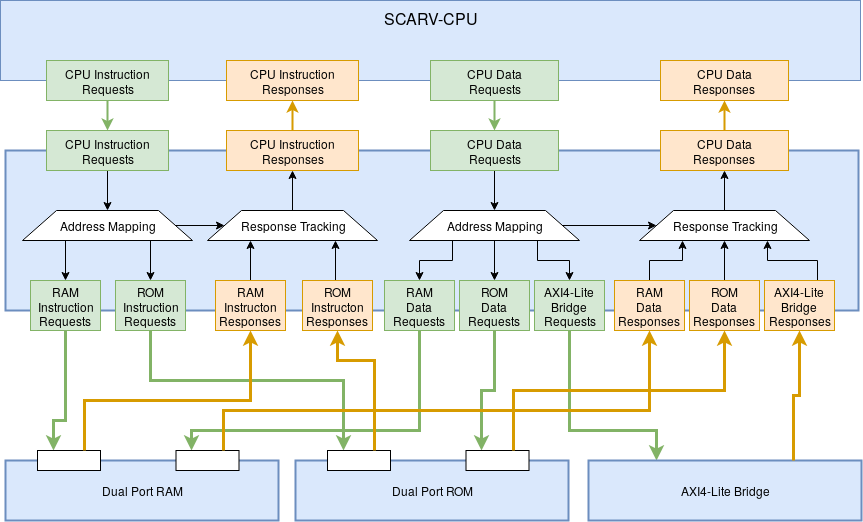
\includegraphics[width=0.8\textwidth]{image/soc-local-ic.png}
\caption{
Block diagram of the \SCARVSOC inner sub-system memory interconnect, 
showing how the \SCARVCPU instruction and data memory requests/responses
are routed to each peripheral.
}
\label{fig:design:soc-local-ic}
\end{figure}

\begin{table}[H]
\centering
\begin{tabular}{lcc}
Peripheral       & \multicolumn{1}{l}{CPU Instruction Memory} & \multicolumn{1}{l}{CPU Data Memory} \\ \hline
Boot ROM         & X                                          & X                                   \\
RAM              & X                                          & X                                   \\
AXI4 Lite Bridge & Unmapped                                   & X
\end{tabular}
\caption{
Table showing which 1st layer peripherals are accessible by the
CPU memory ports.
}
\end{table}

